\chapter{基于手机GPU加速和离线层压缩的能效优化}

%表格模式设置左对齐:
%第一行用\multicolumn{1}{|c|}{文本内容}

本章详细分析了卷积神经网络前向推断过程中所使用基本算子,并对每一个基本算子分别给出了基于手机CPU和手机GPU的实现方式。基于这些基本算子,本章实现了卷积神经网络所需的层结构。然后,利用这些层结构和已训练好的CNN模型权重在手机平台上重构了LeNet和AlexNet,并分析比较了CPU版本和GPU版本两种实现方式的能效。最后,本章描述了基于“剪枝-重训”的权重压缩方法,并使用该方法对卷积神经网络中占存储量主要部分的全连接层权重进行了压缩。对于压缩后的CNN模型,本章进一步使用稀疏矩阵向量乘(SpMV)代替密集矩阵的内积运算,并分别给出了SpMV的CPU和GPU实现方式。

\section{CNN前向推断基本算子的分解与实现}
\label{chapter:chapter3-1}
卷积神经网络的前向推断过程主要涉及卷积层、池化层、全连接层和激活层等的前向传播,故而对CNN前向推断基本算子的分解即需剖析实现这些层所需的基本算子。下面针对每层的基本算子,详细介绍其作用机理并分析比较基于手机CPU和手机GPU实现版本的能效。

\subsection{全连接层基本算子}

\begin{figure}[htbp]
    \begin{center}
    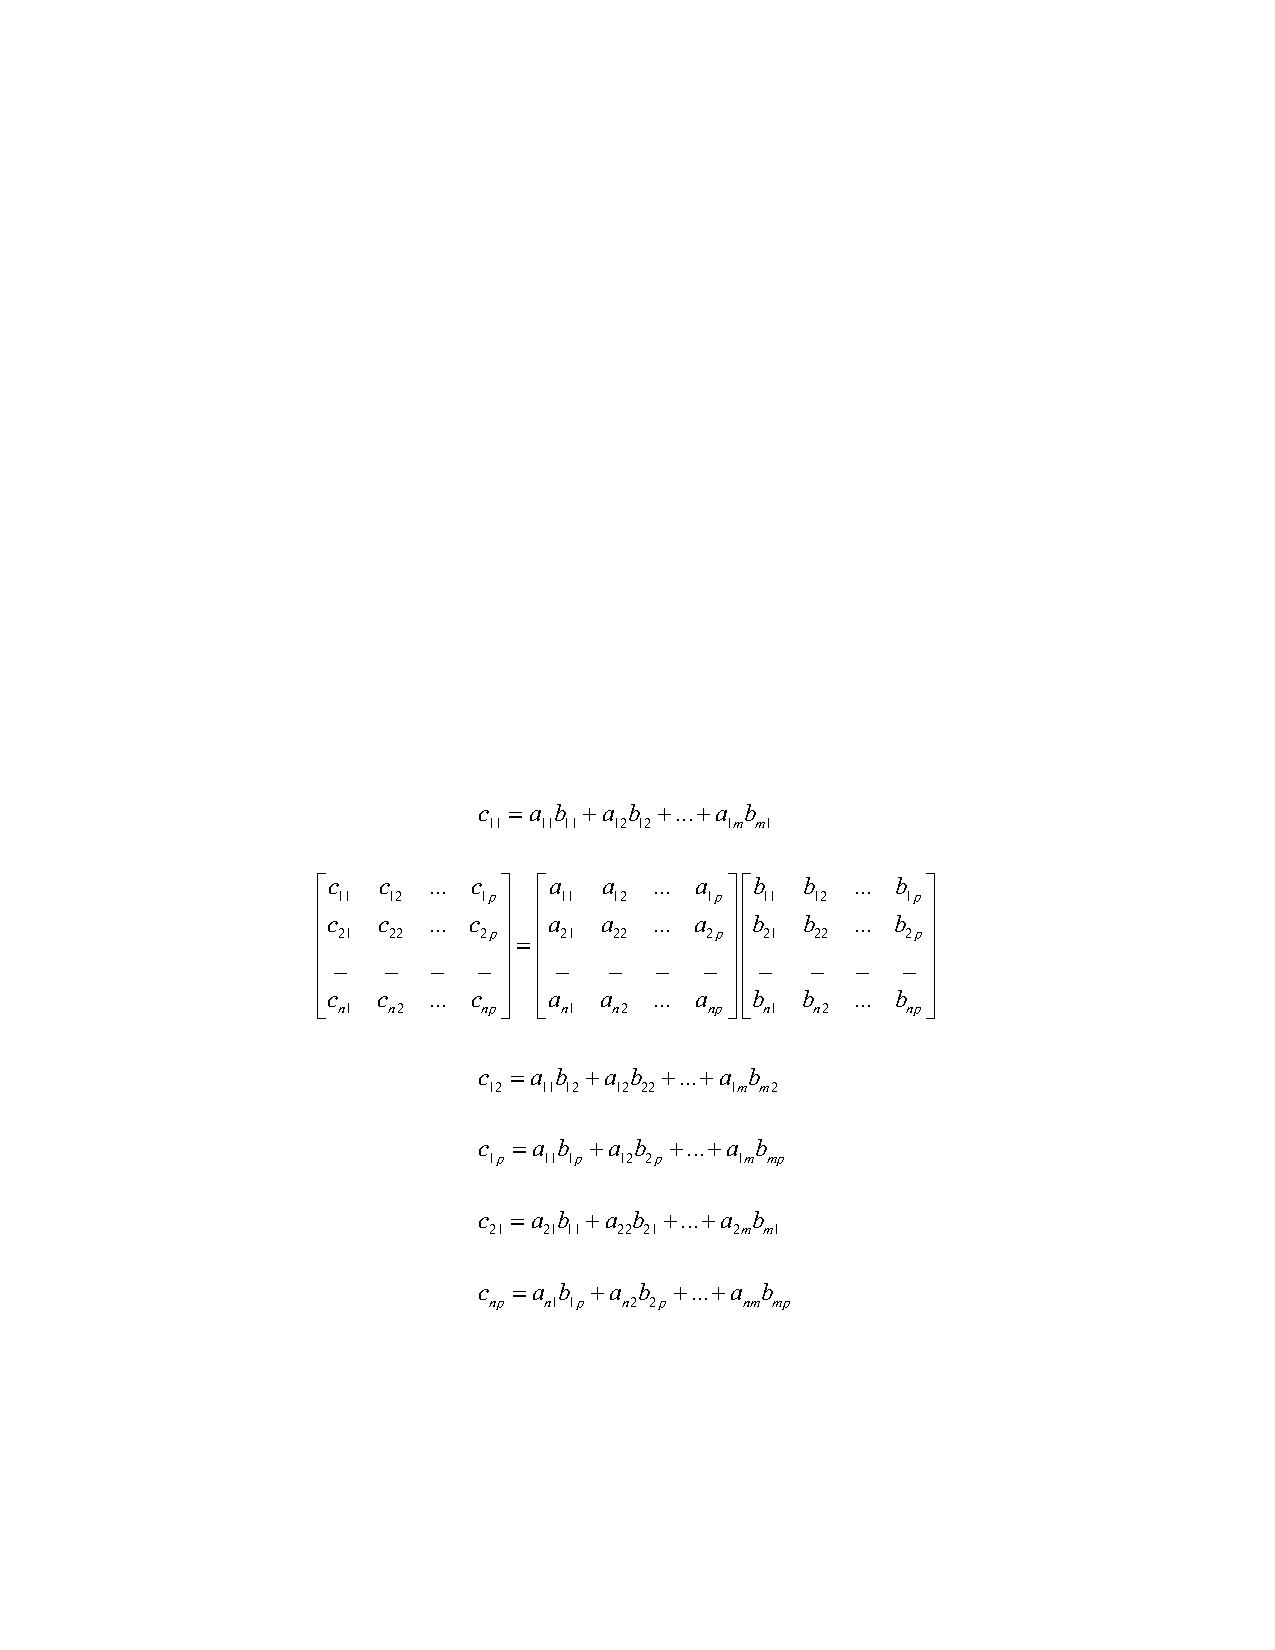
\includegraphics[height=0.5\textwidth]{figures/mat.pdf}
    \end{center}
    \caption{矩阵乘法定义}\label{figure:figure8}
\end{figure}

矩阵乘法操作是全连接层用到的主要基本算子,而在本工作的卷积层实现中其也被涉及,所以在此先介绍矩阵乘法于手机CPU和手机GPU上的实现。图\ref{figure:figure8}给出了矩阵乘法的定义。

根据矩阵乘法的定义可得CPU版本实现的伪代码如下:

\begin{algorithm}[htbp]
	\small
	\SetAlgoLined
	\KwData{mat\_left, row\_left, col\_left, mat\_right, row\_right, col\_right, bias, result}
    \begin{spacing}{0.9}
	\For{i in 0 ... row\_left-1}{
		\For{j in 0 ... col\_right-1}{
            res = 0\;
			\For{k in 0 ... col\_left-1}{
				res +=
				mat\_left[i * col\_left + k] *
				mat\_right[k * col\_right + j]\;
			}
		res += bias[i]\;
        result[i * col\_right + j] = res;
		}
	}
    \end{spacing}
	\caption{CPU版本矩阵乘法}
	\label{algo:algorithm1}
\end{algorithm}

基于OpenCL异构编程框架,下面给出GPU版本的矩阵乘法实现。将CPU版本中第一重和第二重循环的次数分别设置为核函数的全局工作空间大小,可将CPU版本代码直接改成GPU版本的标量形式,伪代码表示如下:

\begin{algorithm}[htbp]
	\small
	\SetAlgoLined
	\KwData{mat\_left, mat\_right, col\_left, bias, result}
    \begin{spacing}{0.9}
    初始化res的值为0\;
	i = get\_global\_id(0)\;
	j = get\_global\_id(1)\;
	col\_right = get\_global\_size(1)\;
	\For{k in 0 ... col\_left-1}{
		res += mat\_left[i * col\_left + k] * mat\_right[k * col\_right + j]\;
	}
    res += bias[i]\;
	result[i * col\_right + j] = res\;
    \end{spacing}
	\caption{GPU版本矩阵乘法(标量形式)}
	\label{algo:algorithm2}
\end{algorithm}

上述伪代码中\texttt{get\_global\_id(dim)}用于获得第\texttt{dim}维上的工作项全局ID,\texttt{get\_global\_size(dim)}用于获得第\texttt{dim}维上的全局工作项个数。GPU版本矩阵乘法的标量形式没有充分利用OpenCL的向量处理能力,这会造成一定的GPU计算性能损失。算法\ref{algo:algorithm3}给出了GPU版本矩阵乘法向量形式的核心伪代码实现。在向量形式实现中使用了\texttt{float4}向量数据类型,并通过API \texttt{dot()}完成对两个\texttt{float4}类型数据的一次内积操作。此处需要注意一点:因为对右矩阵不能使用\texttt{vload4()} API连续读4个数据,所以需要先读取所需的4个数据再将它们转换为一个\texttt{float4}向量类型,这样才能使得两个包含四个元素的向量内积操作可以在一个时钟周期内完成。

\begin{algorithm}[htbp]
	\small
	\SetAlgoLined
	\KwData{mat\_left, mat\_right, col\_left, bias, result}
    \begin{spacing}{0.9}
    初始化res的值为0\;
    remain表示核函数剩余未处理的数据量\;
    \While{remain >= 4}{
        从mat\_left中使用vload函数取出四个数据组成float4向量类型tmp1\;
        从mat\_right中取出与tmp1对应的四个数据组成float4向量类型tmp2\;
        使用dot函数计算res的当前值:res += dot(tmp1, tmp2)\;
        设置mat\_left和mat\_right的下标偏移量\;
        更新剩余未处理的数据量:remain -= 4\;
    }
    \While{remain > 0} {
        从mat\_left中取出一个float数据tmp1\;
        从mat\_right中取出一个float数据tmp2\;
        更新res的当前值:res += tmp1 * tmp2\;
        设置mat\_left和mat\_right的下标偏移量\;
        更新剩余未处理的数据量:remain -= 1\;
    }
    将res加上对应偏置值并将结果赋值给result对应项\;
    \end{spacing}
	\caption{GPU版本矩阵乘法(向量形式)}
	\label{algo:algorithm3}
\end{algorithm}

基于ODROID-XU3实验平台,本文分析比较了上述三个矩阵乘法实现版本的能效。图\ref{figure:figure9}显示了$512\times1024$矩阵与$1024\times512$矩阵相乘的执行时间、能耗和功耗结果。

\begin{figure}[htbp]
    \begin{center}
    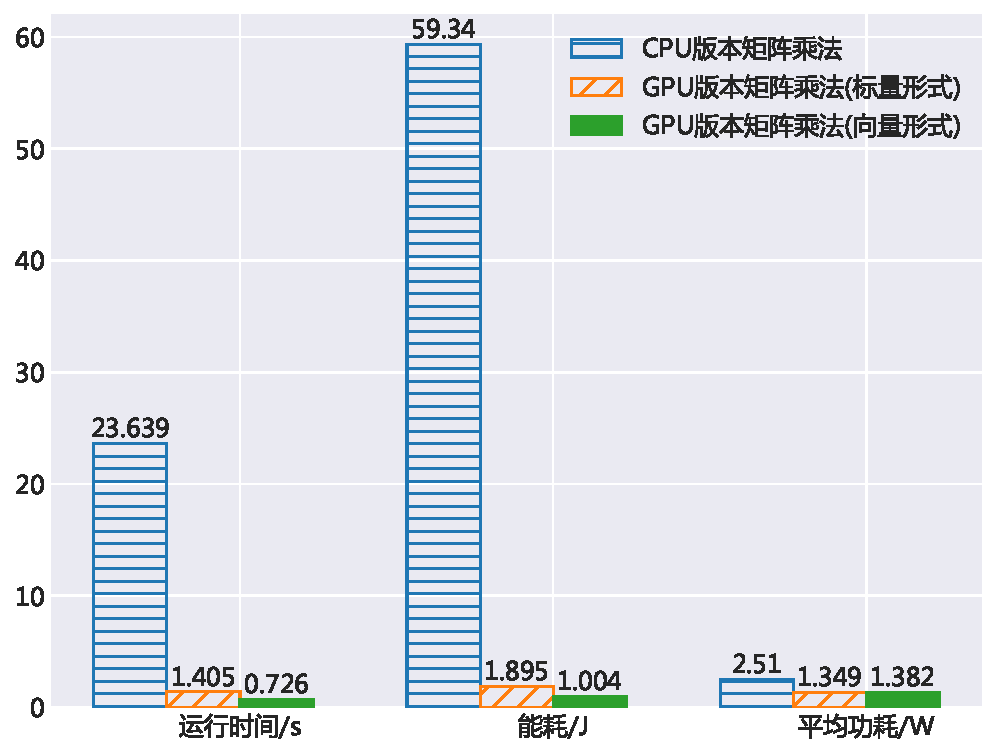
\includegraphics[height=0.4\textwidth]{figures/matmul.pdf}
    \end{center}
    \caption{矩阵乘法不同实现版本的执行时间、能耗和功耗对比}\label{figure:figure9}
\end{figure}

\begin{table}[htbp]
  \centering
  \caption{矩阵乘法不同实现版本的能效对比}
  \label{table:table1}
  \begin{tabular}{cc}
    \toprule
      实现版本 & EDP(Joules*seconds) \\
    \midrule
      CPU版本矩阵乘法 & 1402.763 \\
      GPU版本矩阵乘法(标量形式) & 2.663 \\
      GPU版本矩阵乘法(向量形式) & 0.729 \\
    \bottomrule
  \end{tabular}
\end{table}

由图\ref{figure:figure9}可知,使用手机GPU实现矩阵乘法可以明显提升运算性能并降低运行时能耗和功耗。对于$512\times1024$矩阵与$1024\times512$矩阵的乘积运算,相较于CPU实现版本,GPU的标量实现形式加速比为16.82。另一方面,通过比较GPU版本矩阵乘法的标量实现形式和向量实现形式,可以发现使用OpenCL的\texttt{float4}向量数据类型可以再获得约2倍的性能提升并可进一步降低运行时能耗。由表\ref{table:table1}可知,GPU版本矩阵乘法在能效方面远高于CPU版本矩阵乘法,尤其在使用OpenCL向量数据类型实现时GPU版本的能效提升了近两千倍(EDP的定义见\ref{chapter:edp},其值越小说明能效越高)。

\subsection{卷积层基本算子}

卷积层的基本算子即为卷积操作,这在第二章进行了相关介绍。然而,为了提高卷积操作的执行性能,本章中采用\texttt{img2col}和通用矩阵乘的方式实现卷积操作。

在介绍\texttt{img2col}之前,此处先回顾一下第二章介绍的卷积实现理论细节:卷积核是一个包含权重的小窗口,其在输入图像上按步长滑动,每次滑动会对输入图像上对应的小窗口区域进行操作,即将卷积核中的各个权值与输入图像上对应小窗口中的各个像素值相乘再求和,最后加上偏置得到特征图上的一个输出值。根据上述描述可知,卷积核对输入图的每一次运算与两个向量的内积非常类似。因此,卷积操作完全可以转化为矩阵乘法来实现。为了达到这一目的,需要进行两步操作:(1)使用\texttt{img2col}将输入特征图转换为通过矩阵乘法实现卷积操作时所需的矩阵形式;(2)使用矩阵乘法将权重矩阵与第一步转化而来的矩阵进行相乘以得到卷积输出结果。

\begin{figure}[htb]
    \begin{center}
    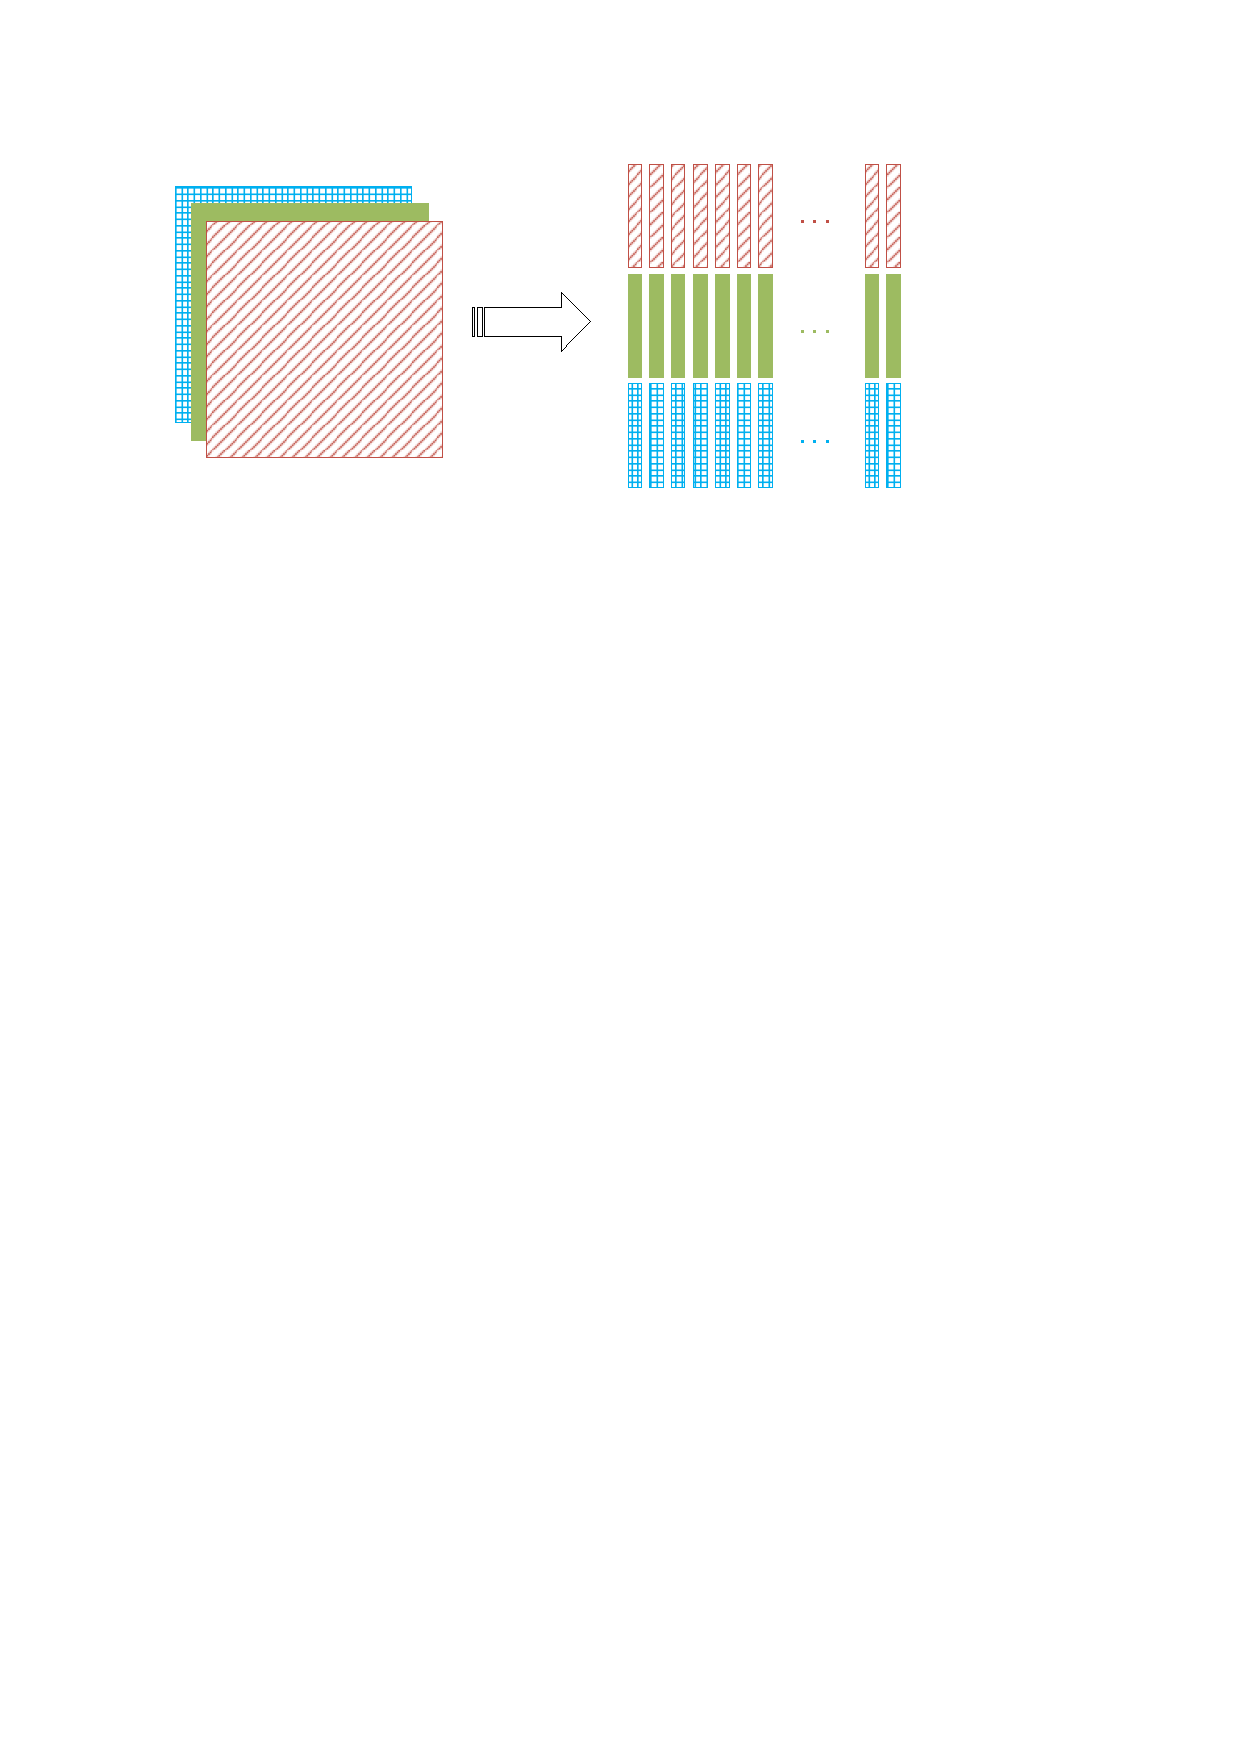
\includegraphics[height=0.25\textwidth]{figures/im2col.pdf}
    \end{center}
    \caption{\texttt{img2col}转换三通道输入特征图示例}\label{figure:figure10}
\end{figure}

图\ref{figure:figure10}给出了一个使用\texttt{img2col}将三通道输入特征图转换为所需输出矩阵的示例,而\texttt{img2col}的执行过程在算法\ref{algo:algorithm4}进行了详细描述。

\begin{algorithm}[htbp]
	\small
	\SetAlgoLined
    \begin{spacing}{0.8}
    \KwData{channels, channel\_size, kernel\_h,kernel\_w, output\_h,output\_w}
    channels,channel\_size分别表示输入通道数和一个通道的数据量\;
    kernel\_h,kernel\_w分别表示卷积核的高度和宽度\;
	output\_h,output\_w分别表示卷积层输出图像的高度和宽度\;
    \For{channel in 0 ... channels-1} {
        \For{kernel\_row in 0 ... kernel\_h-1} {
            \For{kernel\_col in 0 ... kernel\_w-1} {
                计算卷积核中第kernel\_row行在输入图像中的第一个操作区域的行索引\;
                \For{output\_rows in output\_h ... 1} {
                    \If{计算得到的输入图像的行值索引小于零或者大于输入图像的高} {
                        \For{output\_cols in output\_w ... 1} {
                            将该行在输出矩阵上的位置置为0\;
                        }
                    } \Else {
                        计算卷积核中的第kernel\_col列在输入图像中的第一个操作区域的列索引\;
                        \For{output\_col in output\_w ... 1} {
                            \If{输入图像的列值索引大于等于于零或者小于输入图像的宽} {
                                将输入特征图上对应的区域放到输出矩阵上;
                            } \Else {
                                将该行该列在输出矩阵上的位置置为0\;
                            }
                            将输出列坐标移动到下一个卷积窗口\;
                        }
                    }
                    将输出行坐标移动到下一个卷积窗口\;
                }
            }
        }
        将输出矩阵偏移channel\_size以操作下一个输入通道的图像数据\;
    }
    \end{spacing}
	\caption{\texttt{img2col}核心操作伪代码}
	\label{algo:algorithm4}
\end{algorithm}

根据算法\ref{algo:algorithm4}描述的伪代码,本文分别于手机CPU和手机GPU上实现了\texttt{img2col}操作。为了比较\texttt{img2col}在手机CPU和GPU上的执行性能,本文基于ODROID-XU3平台测量了\texttt{img2col}在处理高度和宽度均为256、通道数为100的输入特征图(步长为1,卷积核大小为3)的执行时间、能耗和功耗特征,测量结果如图\ref{figure:figure11}所示。

\begin{figure}[htbp]
    \begin{center}
    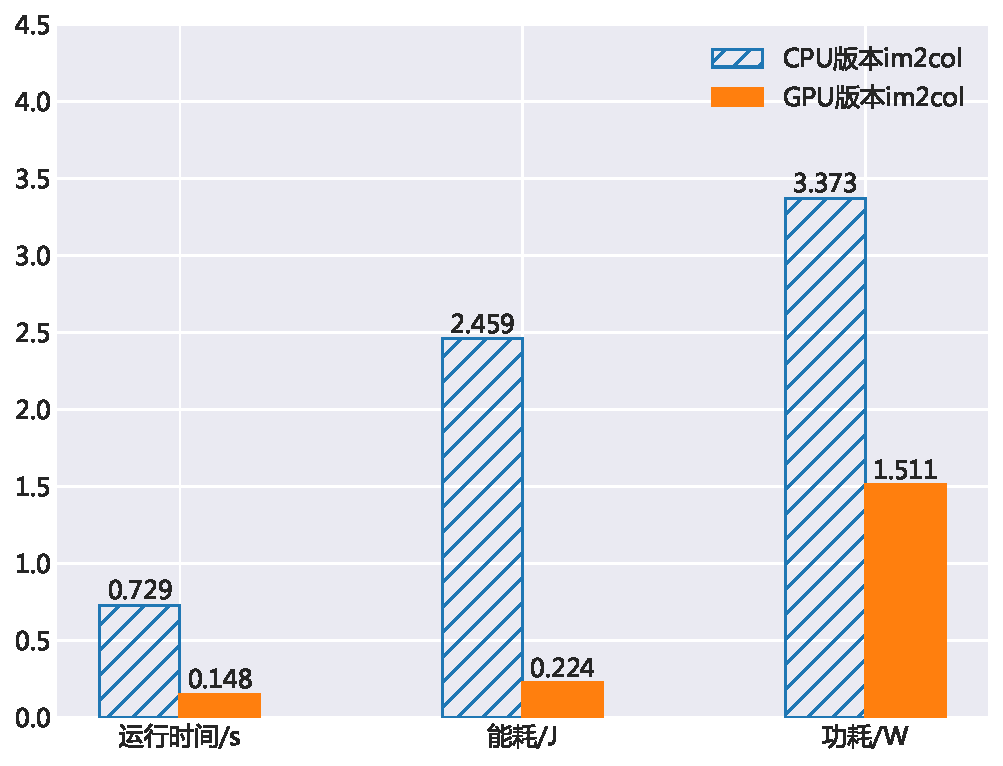
\includegraphics[height=0.4\textwidth]{figures/im2col_energy.pdf}
    \end{center}
    \caption{\texttt{img2col}不同实现版本的执行时间、能耗和功耗对比}\label{figure:figure11}
\end{figure}

由图\ref{figure:figure11}可知,在操作高度和宽度均为256、通道数为100的输入特征图时,相较于CPU版本的\texttt{img2col},GPU版本的\texttt{img2col}可使得执行速度提升5倍左右。与此同时,使用GPU执行\texttt{img2col}操作的能耗仅为使用CPU能耗的1/10,而功耗也降低为使用CPU时的1/2。表\ref{table:table2}显示了GPU版本\texttt{img2col}和CPU版本\texttt{img2col}的EDP值。对比两者的EDP值可知,基于GPU实现的\texttt{img2col}可以将能效提升50倍以上。

\begin{table}[htbp]
  \centering
  \caption{\texttt{img2col}不同实现版本的能效对比}
  \label{table:table2}
  \begin{tabular}{cc}
    \toprule
      实现版本 & EDP(Joules*seconds) \\
    \midrule
      CPU版本im2col & 1.792 \\
      GPU版本im2col & 0.033 \\
    \bottomrule
  \end{tabular}
\end{table}


\subsection{池化层基本算子}

显然,池化层的基本算子即为池化单元。由第\ref{chapter:chapter2-1-2}章节可知,最大池化是目前研究工作中最为常用的池化单元,因此本文主要实现了最大池化操作。根据第\ref{chapter:chapter2-1-2}章节中对最大池化操作的自然语言描述,可形成如算法\ref{algo:algorithm5}所示的最大池化操作伪代码。同样地,本文于手机CPU和手机GPU上分别实现了算法\ref{algo:algorithm5}所描述的伪代码。

对于一张高度和宽度均为256、通道数为100的输入特征图,本文测量了其在ODROID-XU3平台上进行步长为1、池化核大小为3的最大池化操作所需执行时间、能耗和功耗,结果如图\ref{figure:figure12}所示。由图\ref{figure:figure12}可知,使用GPU进行最大池化操作不仅可以将运算速度提升12倍还可以把能耗降为使用CPU时的1/28。最大池化在CPU和GPU上执行的功耗特征与\texttt{img2col}类似,即GPU版本最大池化功耗约为CPU版本最大池化功耗的一半。表\ref{table:table3}从能效的角度分析了最大池化在不同计算设备上的表现,即GPU版本最大池化的能效要高出CPU版本约300余倍。

\begin{algorithm}[htbp]
	\small
	\SetAlgoLined
    \begin{spacing}{0.8}
    \KwData{channels, pooled\_h, pooled\_w}
    channels表示输入通道数\;
    pooled\_h和pooled\_w分别表示池化输出矩阵的高度和宽度\;
    \For{c in 0 ... channels-1} {
        \For{ph 0 ... pooled\_h-1} {
            \For{pw in 0 ... pooled\_w-1} {
                计算本次池化窗口的行操作起始位置hstart和终止位置hend\;
                计算本次池化窗口的列操作起始位置wstart和终止位置wend\;
                确保本次行列操作起始位置hstart和wstart均为非负值\;
                计算本次池化操作输出矩阵的对应下标pool\_index\;
                将本次池化窗口左上角第一个值赋给输出矩阵下标为pool\_index的项\;

                \For{h in hstart ... hend-1} {
                    \For{w in wstart ... wend-1} {
                    	利用上面两重循环遍历本次池化窗口中每一个值value\;
                        将value与输出矩阵下标为pool\_index的项做比较\;
                    	将两者较大值重新赋值给输出矩阵下标为pool\_index的项\;
                    }
                }
            }
        }
        将输入特征图偏与输出矩阵均偏移到下一个通道\;
    }
    \end{spacing}
	\caption{最大池化核心操作伪代码}
	\label{algo:algorithm5}
\end{algorithm}

\begin{figure}[htbp]
\begin{minipage}[b]{.6\linewidth}
    \begin{center}
    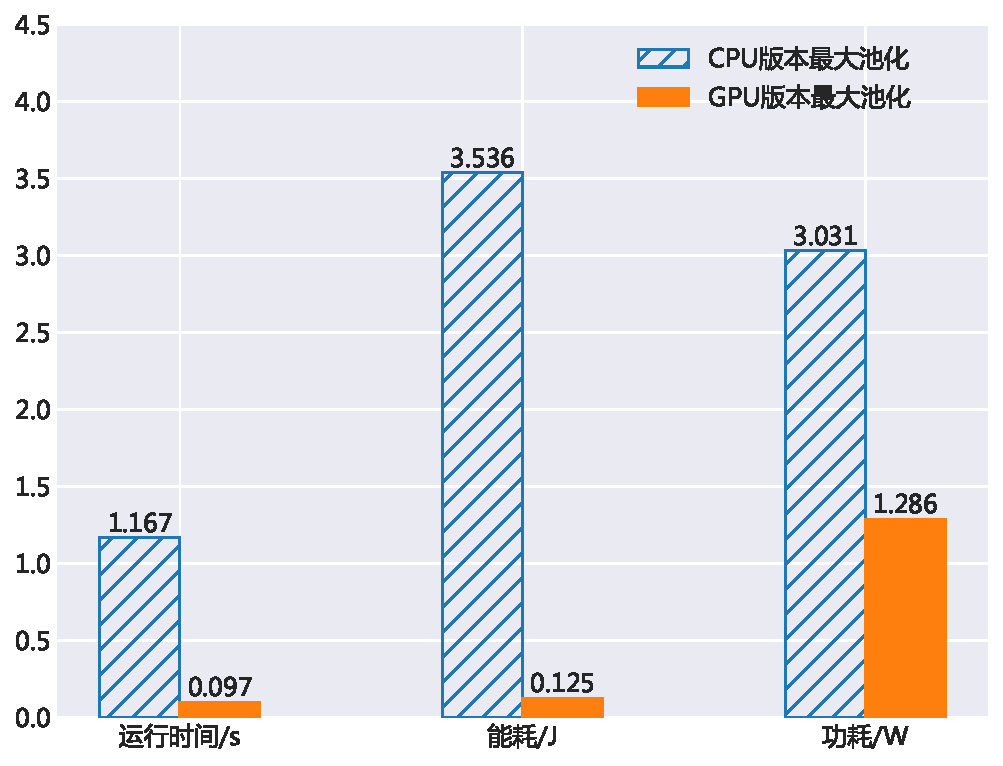
\includegraphics[height=0.65\textwidth]{figures/pool_energy.pdf}
    \end{center}
    \captionsetup{font={small}}
    \caption{最大池化不同实现版本的执行时间、\\能耗和功耗对比}\label{figure:figure12}
\end{minipage}
\begin{minipage}[b]{.4\linewidth}
\centering
\resizebox{1.0\textwidth}{!}{
\begin{tabular}{cc}
    \toprule
      实现版本 & EDP(Joules*seconds) \\
    \midrule
      CPU版本最大池化 & 4.125 \\
      GPU版本最大池化 & 0.012 \\
    \bottomrule
\end{tabular}
}
\captionsetup{font={small}}
\captionof{table}{最大池化不同实现版本的\\能效对比}\label{table:table3}
\end{minipage}
\end{figure}

%\begin{figure}[htb]
%    \begin{center}
%    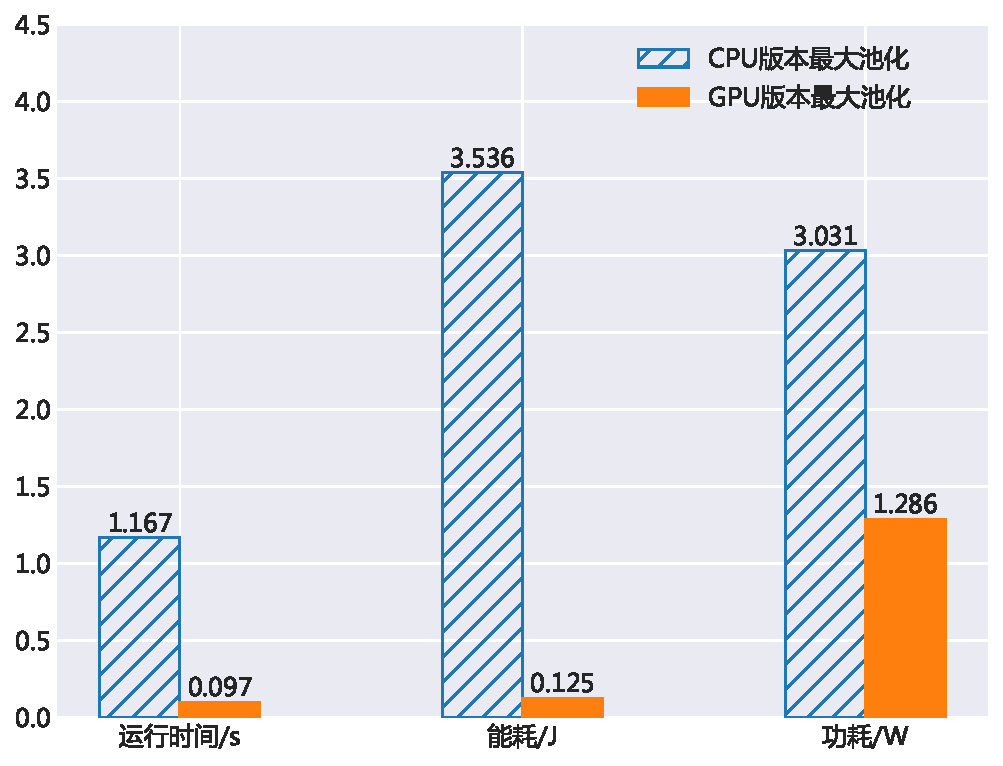
\includegraphics[height=0.4\textwidth]{figures/pool_energy.pdf}
%    \end{center}
%    \caption{最大池化不同实现版本的执行时间、能耗和功耗对比}\label{figure:figure12}
%\end{figure}
%
%\begin{table}[htbp]
%  \centering
%  \caption{最大池化不同实现版本的能效对比}
%  \label{table:table3}
%  \begin{tabular}{cc}
%    \toprule
%      实现版本 & EDP(Joules*seconds) \\
%    \midrule
%      CPU版本最大池化 & 4.125 \\
%      GPU版本最大池化 & 0.012 \\
%    \bottomrule
%  \end{tabular}
%\end{table}

\subsection{激活层基本算子}

正如第\ref{chapter:chapter2-1-4}章节所述,激活层主要使用非线性激活函数对输入数据进行处理,故而激活层的基本算子即为所使用的激活函数。在具体实现中,可选的激活函数主要有Relu函数、Sigmod函数以及双曲正切函数等。选定激活函数\texttt{activation\_fun()},激活层基本算子的实现伪代码可表示如下:

\begin{algorithm}[htbp]
	\small
	\SetAlgoLined
	\KwData{data, length}
	\For{i in 0 ... length-1}{
        data[i]=activation\_fun(data[i])\;
	}
	\caption{激活层基本算子实现伪代码}
	\label{algo:algorithm6}
\end{algorithm}

根据算法\ref{algo:algorithm6}所描述的实现逻辑,本文分别实现了基于手机CPU和手机GPU的激活操作。图\ref{figure:figure13}显示了Relu激活算子分别于手机CPU和手机GPU上处理$100 \times 256 \times 256 $个输入数据时的执行时间、能耗和功耗。可以看出,在输入数据量为$100 \times 256 \times 256 $时,GPU版本Relu激活算子的执行速度可比CPU版本的快6倍,并同时可降低22倍的能耗和3.5倍的功耗。表\ref{table:table4}给出Relu激活算子分别在CPU和GPU上运行时的能效。其中,CPU版本Relu激活算子的EDP为0.034,而GPU版本Relu激活算子的EDP仅为0.0003。根据EDP值越小能效越高的度量标准可知,在输入数据量为$100 \times 256 \times 256 $时,Relu激活算子在GPU上的运行时能效是其在CPU上运行时能效的100多倍。

\begin{figure}[htbp]
\begin{minipage}[b]{.6\linewidth}
    \begin{center}
    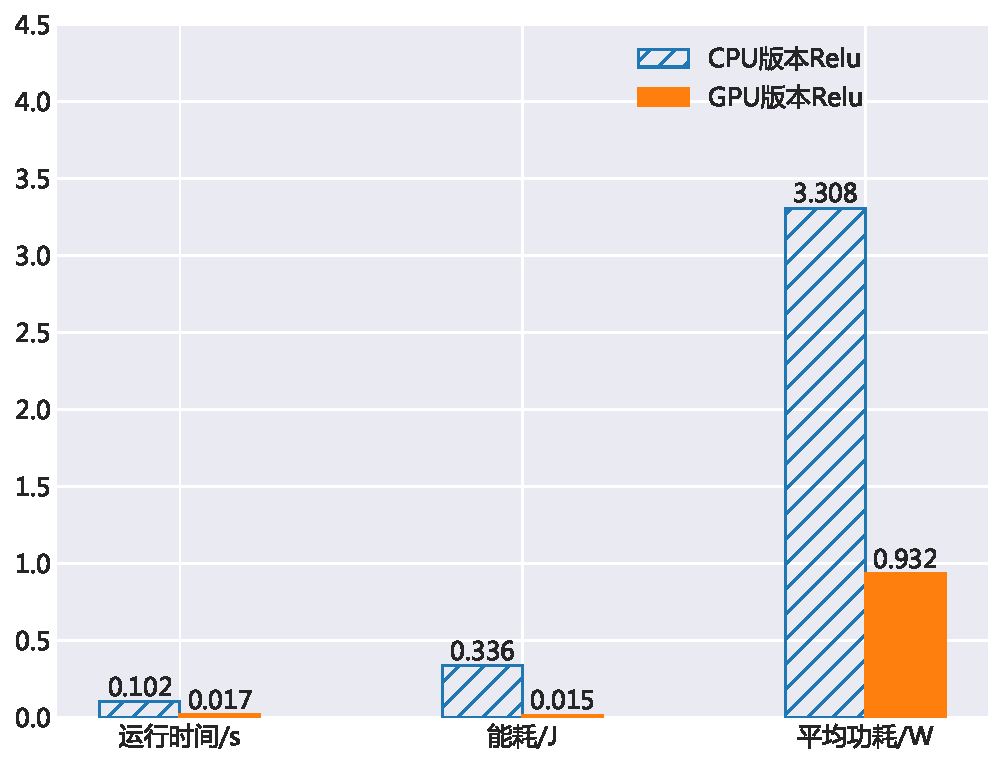
\includegraphics[height=0.65\textwidth]{figures/relu_energy.pdf}
    \end{center}
    \captionsetup{font={small}}
    \caption{Relu激活算子不同实现版本的执行时间、\\ 能耗和功耗对比}\label{figure:figure13}
\end{minipage}
\begin{minipage}[b]{.4\linewidth}
\centering
\resizebox{1.0\textwidth}{!}{
\begin{tabular}{cc}
    \toprule
      实现版本 & EDP(Joules*seconds) \\
    \midrule
      CPU版本Relu激活算子 & 0.034 \\
      GPU版本Relu激活算子 & 0.0003 \\
    \bottomrule
\end{tabular}
}
\captionsetup{font={small}}
\captionof{table}{ Relu激活算子不同实现版本的能效对比}\label{table:table4}
\end{minipage}
\end{figure}

\section{基于手机GPU加速的CNN前向推断}

第\ref{chapter:chapter3-1}章节对卷积神经网络前向推断过程中所涉及的基本算子进行了分解与实现,而本章节即利用这些基本算子分别实现了基于手机GPU和手机CPU的CNN前向推断过程所需层结构,包括卷积层、池化层、全连接层和激活层等。利用所实现的各种层结构,本章节于手机端重构了LeNet和AlexNet模型,并分析比较了两个模型在手机GPU和手机CPU上运行时的能效特征。

\subsection{预训练CNN模型权重参数解析}
\label{chapter:chapter3-2-1}
解析预训练CNN模型权重参数是在手机端重构卷积神经网络前向推断过程的首要条件,本文针对Caffe、YOLO以及Tensorflow等深度学习框架所训练的CNN模型给出了权重解析的python脚本。该脚本可以提取预训练CNN模型的每层权重参数(权值矩阵和偏置矩阵等),并将这些权重参数分层保存为二进制npy文件格式,整个流程如图\ref{figure:figure14}所示。

\begin{figure}[htbp]
    \begin{center}
    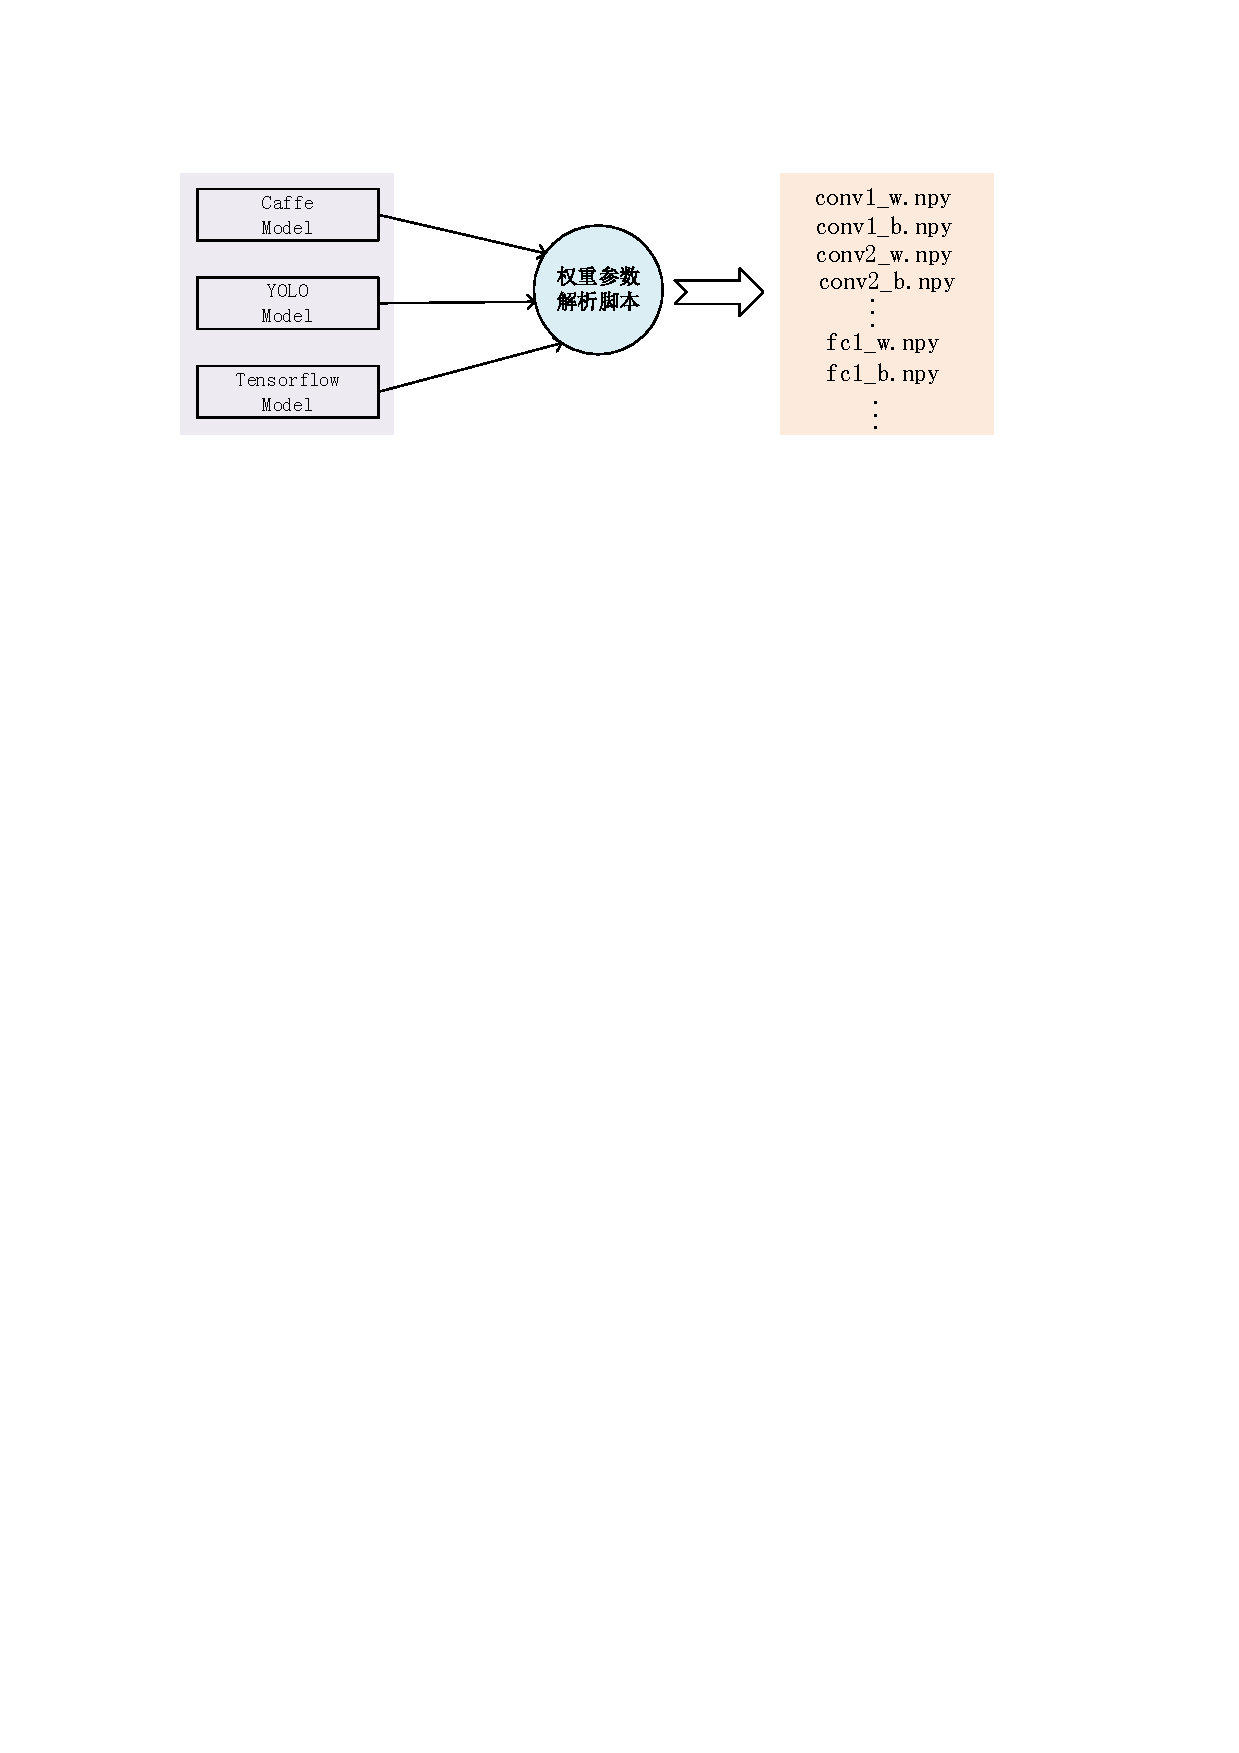
\includegraphics{figures/weight.pdf}
    \end{center}
    \caption{CNN模型权重参数解析流程概览}\label{figure:figure14}
\end{figure}

\subsection{LeNet模型于手机端的重构}

LeNet是由卷积神经网络之父Yan LeCun提出的,其主要用来进行手写字符的识别与分类。

\begin{table}[htbp]
  \centering
  \caption{LeNet模型结构中的卷积层和全连接层}
  \label{table:table5}
\resizebox{1.0\textwidth}{!}{
  \begin{tabular}{ccc}
    \toprule
      名称 & 类型 & 描述\\
    \midrule
      conv1 & 卷积层 & 输入:1x28x28,卷积核:20x1x5x5,步长:1,padding:0,输出:20x24x24 \\
      conv2 & 卷积层 & 输入:20x12x12,卷积核:50x20x5x5,步长:1,padding:0,输出:50x8x8\\
      ip1 & 全连接层 & 输入:800, 输出:500 \\
      ip2 & 全连接层 & 输入:500, 输出:10 \\
    \bottomrule
  \end{tabular}
}
\end{table}


\subsection{AlexNet模型于手机端的重构}









